%% TCC - Monografia
%% Ci\^{e}ncia da Computa\c{c}\~{a}o - LCMAT - CCT - UENF, 2018
%%  


\chapter{Introdu\c{c}\~{a}o}

As possibilidades que sugiram com as tecnologias oriundas na era da Web 2.0, como por exemplo as diversas formas de criar, compartilhar e interagir entre os usuários. \citeonline{SueBennet2011} destaca que as chamadas mídias sociais se tornaram uma ferramente onde cada usuário pode coletivamente ou individualmente publicar e compartilhar imagens, arquivos em diversos formatos, como áudio, vídeo e texto.

As possibilidades são inúmeras com a Web 2.0, que traz consigo padrões comuns de arquitetura, há muitas informações sobre essas arquiteturas no artigo de \citeonline{Governor2009} que aborda diversos conceitos e modelos que utilizamos hoje e muitas das vezes não sabemos os nomes, como por exemplo: \textbf{Service-Oriented Architecture (SOA)}, \textbf{Software as a Service (SaaS)}, \textbf{Participation-Collaboration}, \textbf{Asynchronous Particle Update}, \textbf{Mashup}, \textbf{Rich User Experience (RUE)}, \textbf{The Synchronized Web}, \textbf{Collaborative Tagging, Declarative Living and Tag Gardening}, \textbf{Semantic Web Grounding}, \textbf{Persistent Rights Management} e  \textbf{both adopters of this pattern}. Nesse momento não é necessário saber as definições, mas buscar compreender que existiu uma mudança muito significativa na transição da Web 1.0 para a Web 2.0 e essa mudança nos trouxe termos novos e outros que já não eram mais utilizados.

Os padrões de iteração, compartilhamento, leitura e postagem em massa, trouxe uma outra perspectiva de como projetar software. Por tempos a área da engenharia de software foi espelho das engenharias tradicionais, entretanto o desenvolvimento de software se difere tanto nos processo, quanto nos projetos arquitetônicos de software. Durante essa revolução de técnicas e tecnologias os antigos conceitos já bem definidos pelo meio cientifico como o de sistemas distribuídos, voltaram a reaparecer de forma repaginada como \citeonline{Richards2015}.

É comum os desenvolvedores iniciarem seus projetos sem pensar na arquitetura que será aplicada a aquele projeto. É natural desenvolver um sistema utilizando a arquitetura em camadas, comumente chamada também de arquitetura monolítica. Porém segundo \citeonline{Richards2015} não se deve pensar que qualquer problema poderá ou deve ser resolvido com apena uma arquitetura e para saber a melhor arquitetura para aquele projeto, é necessário conhecer diversos exemplos e quando utilizar.

 
 No capítulo 2 serão destacadas algumas informações sobre as arquiteturas de software como \cite{Tanenbaum1944}, \cite{Richards2015} e \cite{Chiaradia2018} descrevem em seus livros. Mas é importante estar ciente que o escopo deste trabalho será apresentar duas arquiteturas, são elas a arquitetura baseada em \textbf{microsserviços} e arquitetura em \textbf{camadas/monolítica}, pois são as mais populares e a que desejamos buscar mais informações.

\section{Problema}

\citeonline{Schmidt2018} disserta que os softwares modernos que consiste diversas \textbf{features}(funcionalidades), a cada nova funcionalidade é natural que o grau de complexidade do software aumente, não bastando a complexidade aumentar, há outros fatores como: a falta de organização da arquitetura de pastas, códigos difíceis e altamente acoplados entre si e, complexidade para dar manutenção e \textbf{refatoração}. Diante de todas as características é importante entender, segundo \cite{Schmidt2018} que cria-se uma dificuldade para que outros engenheiros de software ou programadores consigam entender o design, a estrutura e as dependências que fazem parte daquela arquitetura.

\cite{Richards2015} cita que o padrão arquitetural natural de desenvolvimento de software e o que a maioria das organizações tradicionais aplicam para todos os projetos e problemas, também tem suas desvantagens e uma delas é ser difícil se manter, refatorar ou até modificar o código. Adicionar novas funcionalidades a um sistema já existente sem ponderar as variáveis e a melhor arquitetura para aquele projeto resultará em um colapso, segundo \cite{Schmidt2018}.

Uma arquitetura baseado em camadas como na \ref{fig:open-layer} tem camadas extremamente acopladas, cada parte é responsável por uma determinada ação na arquitetura. Como \cite{Richards2015} explana, a arquitetura em camadas tende a se tornar complexa, difícil de manter à longo prazo, deploys lentos, testes automatizados lentos e um alto custo para escalar em alguns cenários a aplicação.

\begin{figure}[htbp]
    \hypertarget{arquitetura-camadas}{%
        \caption{Arquitetura em camadas e o seu fluxo}
        \begin{center}
          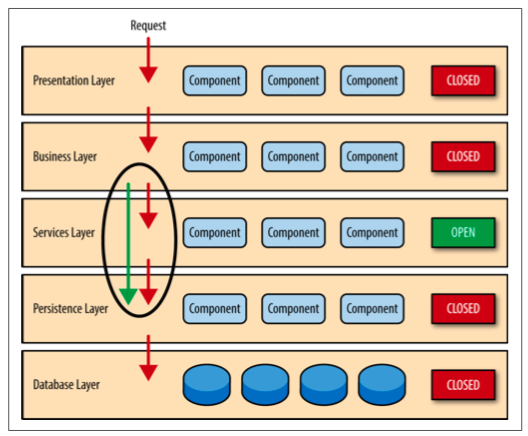
\includegraphics[width=10cm]{Monografia-FormatoLatex/Imagens/open-layer.png}
        \end{center}
    }
    \legend{Fonte: Imagem retirada do livro \citeonline[Cap.~1]{Richards2015}}.}}
    \label{fig:open-layer}
\end{figure}


\section{Hipótese}

A arquitetura baseada em Microsserviços:
\begin{itemize}
    \item Implementação arquitetural rápida
    \item Escalar a aplicação de forma fácil e com diminuição de custos
    \item Fácil manutenabilidade
    \item Fácil utilização de várias linguagens de programação
    \item Deploy rápido e fácil
    \item Logs difíceis de manter
    \item Fácil implementação de autorização e autenticação
\end{itemize}

\section{Objetivo Geral}

O objetivo do trabalho é implementar e verificar o quão complexo é implementar as arquiteturas em camadas e a baseada em microsserviços e analisar a escalabilidade, manutenibilidade, o uso de multi tecnologias, a facilidade do deploys, a verificação dos logs, implementação e manutenção da autorização e autenticação nas duas arquiteturas e fazer uma comparação empírica entre ambas.

\section{Justificativa}

Com o avanço das tecnologias os engenheiros precisam estar preparados para lidar com problemas arquiteturais complexos, haja visto a complexidade dos sistemas que estamos desenvolvendo hoje em dia. \cite{Schmidt2018} explana o quanto precisamos entender melhor sobre as arquiteturas, tanto as vantagens, quanto as desvantagens. Com o desenvolvimento dos softwares modernos e com softwares cadas vez mais distribuídos em conceitos como \textbf{cloud}, infra-estrutura e plataforma como serviço, precisamos de mais estudos científicos sobre as arquiteturas e mais especificamente a baseada em microsserviços, não é uma arquitetura nova, porém é uma evolução de modelos antigos para os sistemas de hoje.

Há inconvenientes quando se implementa uma arquitetura em camadas sem se planejar, como já dito suas vantagens e desvantagens devem ser levadas em consideração e também o projeto e equipe. \cite{Schmidt2018} propõe que os arquitetos e os engenheiros devem entender todas as características das diversas arquiteturas que já foram catalogadas. Há poucos artigos cientifico sobre arquiteturas de modo geral e também especificamente sobre a arquitetura baseada em microsserviços.

O aprendizado em arquitetura e a experiência sobre softwares mal planejados fazem com que esse trabalho seja importante para entender melhor as arquiteturas propostas nesse projeto. Esse trabalho é importante não só para a formação, mas pela identificação com essa temática da engenharia de software.


\section{Método}

Para o proposito deste trabalho será estabelecido o estudo da arquitetura de microsserviços, analisando todo o fluxo entre as partes que compõe as arquiteturas.A implementação é uma parte fundamental desse trabalho, haja visto que com as implementações feitas, poderemos obter dados empírico e também dados analíticos.

Dito o resumo acima o método utilizado será:
 \begin{itemize}
     \item Levantamento bibliográfico sobre os tópicos abordados neste trabalho como: Arquiteturas, Microsserviços, Sistemas distribuídos e outros;
     \item Pesquisar sobre a Arquitetura de Microsserviços  e sua implementação;
     \item Definição das ferramentas para a construção da arquitetura de Microsserviços;
     \item Escolha das tecnologias;
     \item Modelagem da arquitetura pensando nas ferramentas e nas vantagens da ferramenta;
     \item Implementação da arquitetura com a utilização das tecnologias Open Source;
     \item Com um navegador analisar o tempo de requisição e resposta. Relatar o esforço para a implementação de ambas as arquiteturas. Efetuar testes no desligamento do servidor e analisar como se comporta o sistemas.
     \item Testar e documentar os resultados
 \end{itemize}
